\documentclass[]{scrartcl}

\usepackage{geometry}
 \geometry{
    a1paper,
    left=40mm,
    right=40mm,
    top=40mm,
    bottom=40mm
}

\pagestyle {empty}

\usepackage{graphicx, epsfig}
\usepackage[inkscapeformat=png]{svg}
\usepackage{rotating} 
\usepackage{caption}
\usepackage{float} 

% настройка шрифтов и языков
\usepackage[english, russian]{babel} % для работы с английским и русским языками
\usepackage[T2A]{fontenc} % для норм паказа символов в pdf
\usepackage[utf8]{inputenc} % для норм взаимодействия символов для самого tex

\usepackage{fontspec} % для работы со шрифтами 
\usepackage{polyglossia} % Поддержка многоязычности
\defaultfontfeatures{Ligatures=TeX,Mapping=tex-text}

\setmainlanguage[babelshorthands = true]{russian} 
\setotherlanguage{english} 
\setmainfont{Times New Roman} 
\newfontfamily\cyrillicfont[Script=Cyrillic]{Times New Roman} 
\newfontfamily\englishfont{Times New Roman} 

\begin{document}
  \begin{sidewaysfigure}
    \centering
    \def\svgwidth{\textwidth}
    \caption*{\englishfont \cyrillicfont \bfseries \fontsize{70pt}{70pt}\selectfont СТРУКТУРА ЯЧЕЙКИ КЛАССИЧЕСКОЙ LSTM СЕТИ}
    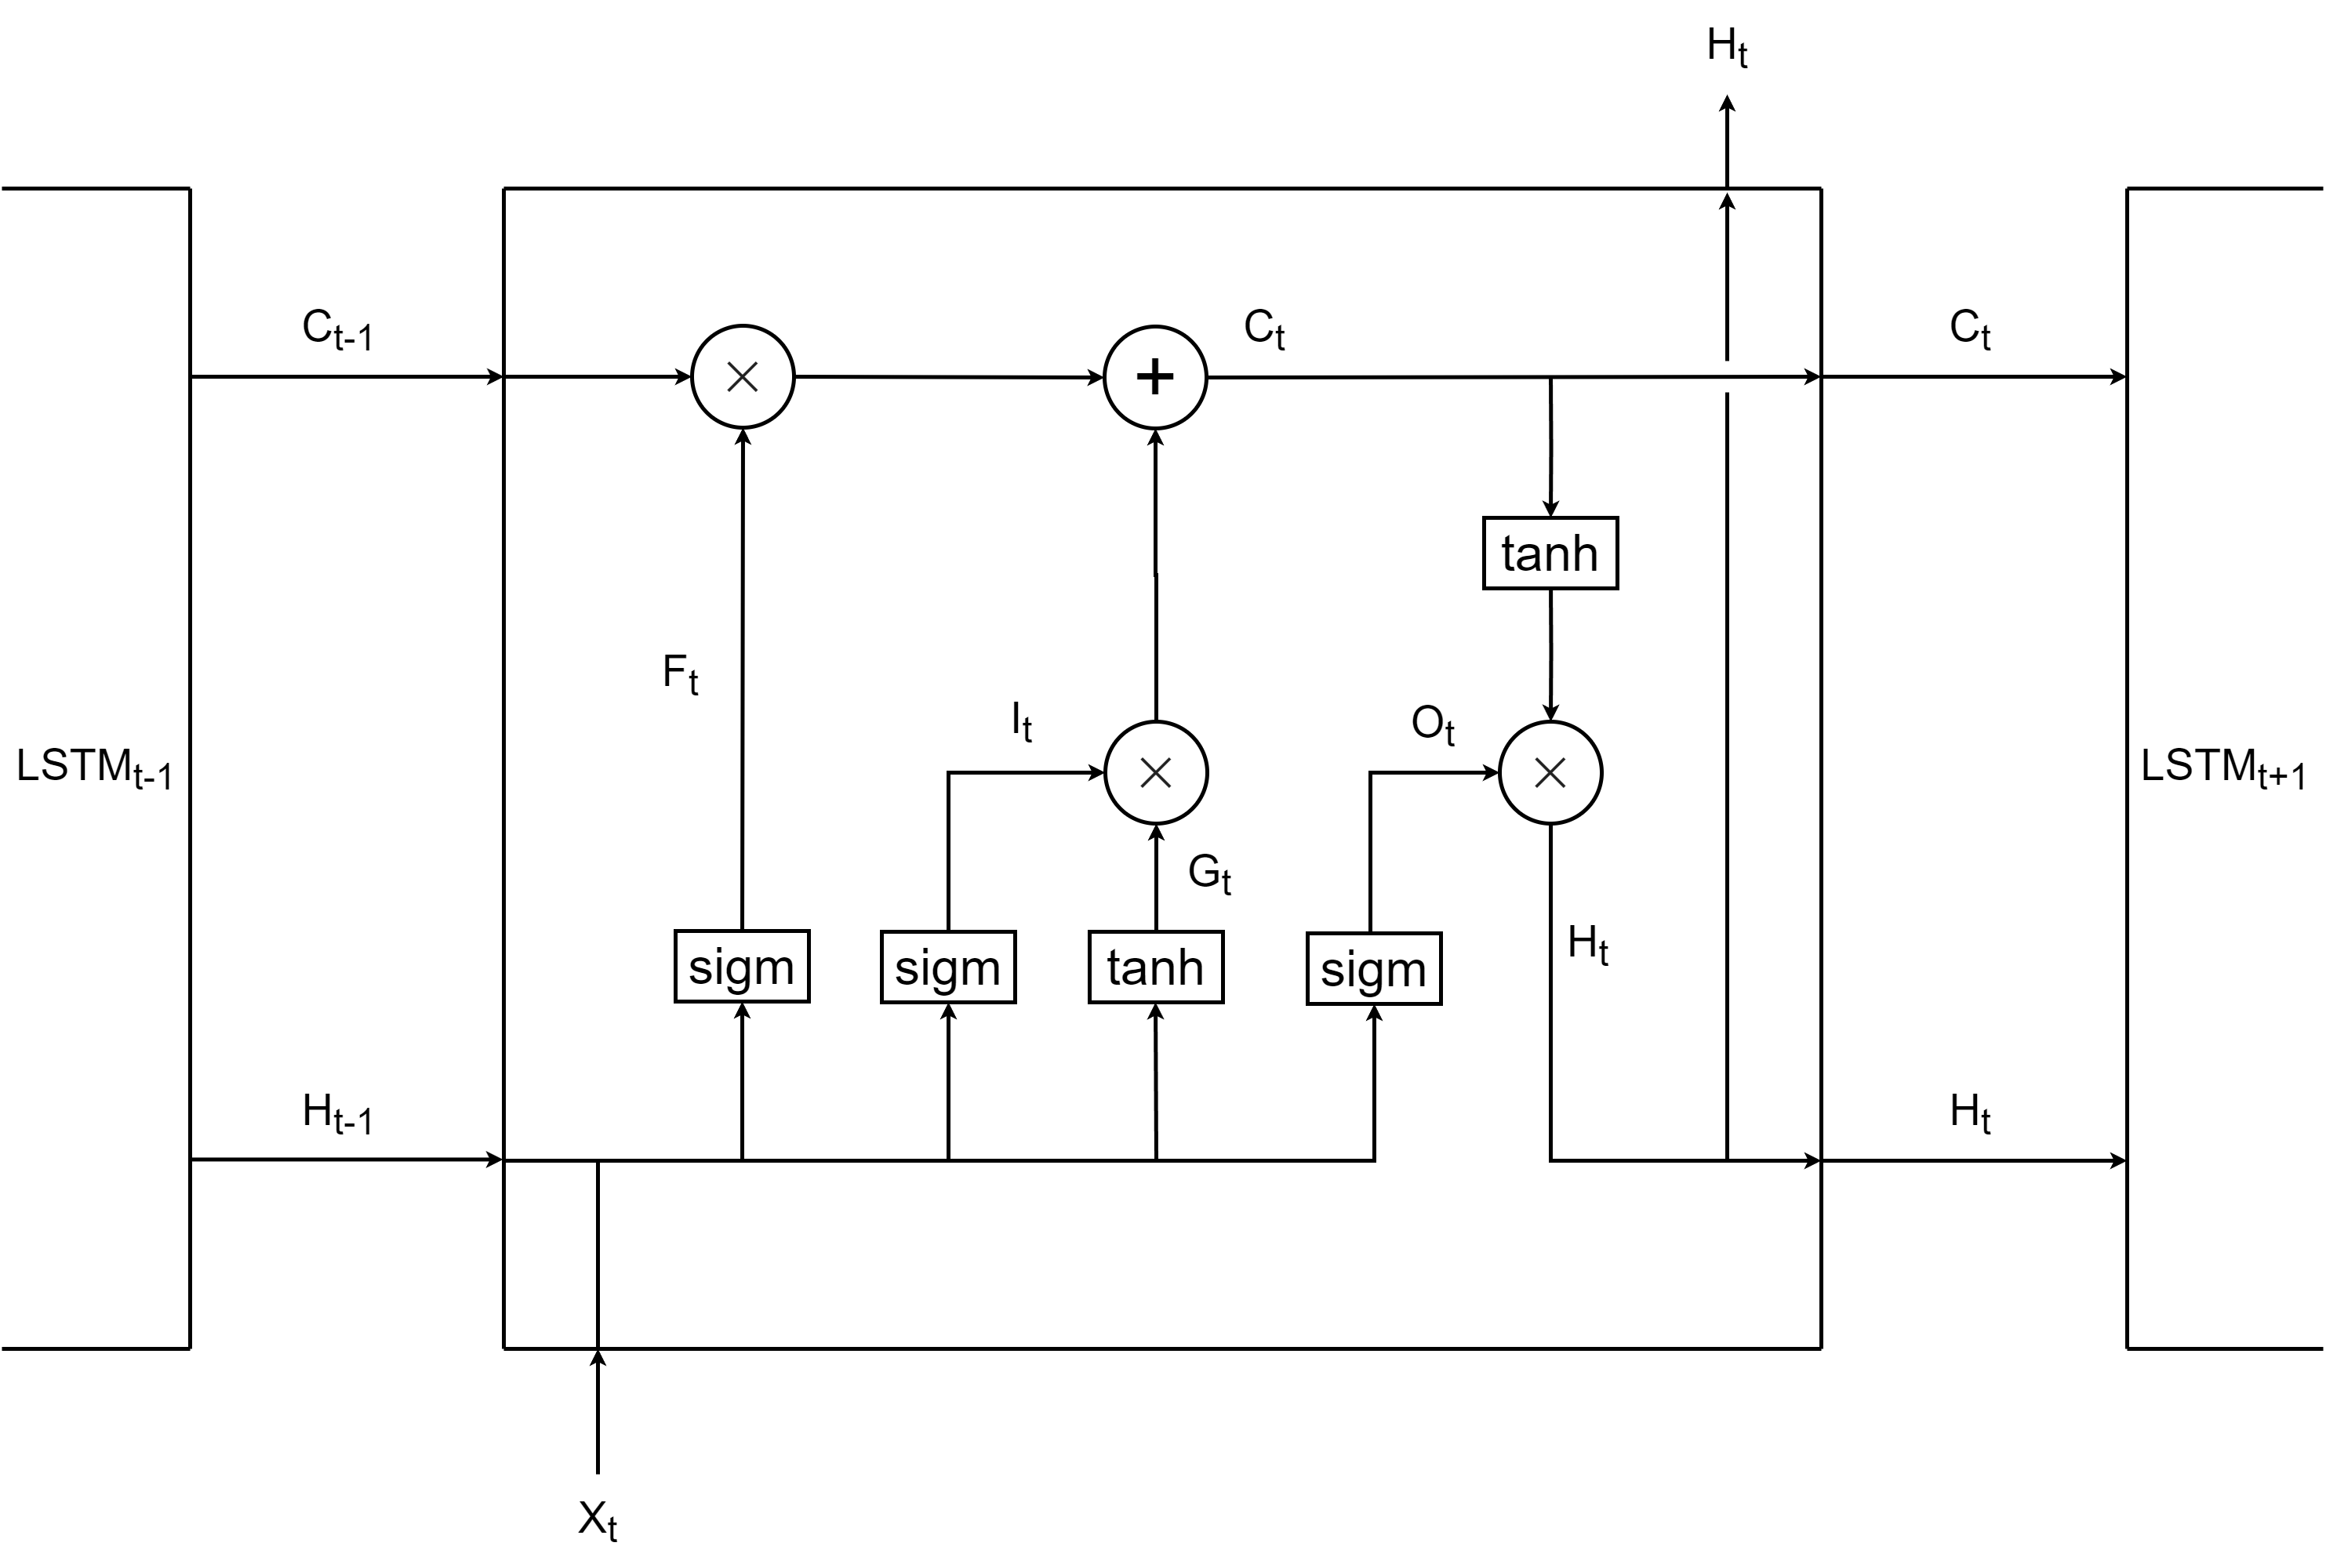
\includegraphics[width=\textheight]{LSTM.png}
    \label{fig:PUS}
  \end{sidewaysfigure} 
\end{document}